\section{Introduction \label{sec:intro}}

%Neutrino oscillation experiments provide a window on to beyond the standard model physics of neutrino mass generation
% by measuring the properties of the neutrino mixing matrix and mass splittings.  The first observation of a 
%neutrino appearance signal by T2K~\cite{t2knue} has
% opened the door for the determination of the neutrino mass hierarchy and CP phase at current (T2K, NO$\nu$A) 
%and proposed (Hyper-K, LBNF, LBNO) long baseline accelerator experiments.  To make precision measurements of 
%oscillations parameters, including the CP violating phase, future experiments must achieve systematic uncertainties on 
%neutrino event rate predictions at the 2\% level or better.  In the current T2K $\nu_{e}$ appearance measurement, 
%the combined uncertainty on the neutrino flux and interaction modeling is 8\%, even with the constraint from 
%near detector data.  Significant improvements are needed to reach the level necessary for precision oscillation measurements.

Now that neutrino appearance has been observed by the T2K experiment~\cite{t2knue}, it is possible to determine the 
neutrino mass hierarchy and CP phase with current (T2K~\cite{Abe:2014tzr}, NO$\nu$A)  and proposed (Hyper-K~\cite{Abe:2011ts},
 LBNF, LBNO) long baseline 
accelerator experiments.  To make precision measurements of neutrino mixing parameters, including the CP violating phase, 
future experiments must achieve systematic uncertainties on neutrino event rate predictions at the 2\% level or better.  
The current T2K $\nu_{e}$ appearance measurement, the combined uncertainty on the neutrino flux and interaction modeling is 8.8\%.  
Significant improvements are therefore needed to reach the level necessary for precision oscillation measurements.

Substantial reduction to the overall systematic uncertainty is typically provided through the use of a near detector, 
which measures the initial rate of neutrino interactions prior to oscillation, however there are limitations to this technique 
as it is used currently.  First, the near detector measures abundant $\nu_\mu$ interactions to predict the oscillated $\nu_{e}$ 
event rate. In the T2K analysis, 3\% of the total uncertainty is based on theory calculations of the ratio of $\nu_{e}$ to $\nu_{\mu}$ 
cross sections; it is difficult to directly measure with comparable precision at the near detector as the $\nu_{e}$ component of 
the flux is significantly smaller by design. Second, uncertainties associated with the modeling of nuclear effects in neutrino 
interactions are significant in the T2K analysis; 7.5\% are uncertainties which do not cancel in the extrapolation. Third, 
reports of non-standard physics, such as sterile neutrinos, would modify the near detector event rate and affect the 
extrapolation; alternate explanations such as nuclear effects would also be relevant for the long baseline program.

In recent years, the incorporation of nuclear effects into the modeling of
neutrino interactions at the GeV scale has been a significant challenge.  The MiniBooNE 
"excess" of CCQE-like $\nu_{\mu}$ candidate events, particularly at large $Q^{2}$, 
has been interpreted as previously un-modeled nuclear effects which produce multi-nucleon final states with
no final state pions.  However, attempts to calculate these nuclear effects have provided disparate results, and there
is still no model that postdicts all of the experimental data.  Uncertainties associated with the
modeling of nuclear effects in neutrino interactions are expected to be a dominant systematic uncertainty
for future neutrino oscillation measurements.

Even if a model can correctly postdict observed event rates and kinematic distributions for a particular 
measurement an ambiguity often remains because the broad energy spectrum of neutrinos in neutrino beam presents
an under-constrained problem, {\it ie.} it is not possible to find a unique solution for the energy dependent 
neutrino interaction rate and final state particle kinematics that satisfies the data.  In one approach, the
under-constrained problem is addressed by combining constraints from different experiments with spectra peaked
at different energies.  However, the effectiveness of this approach can be limited due to systematic differences in 
measurements from multiple experiments.  A recent example is the seeming discrepancy in pion production spectra measured
by MiniBooNE and MINER$\nu$A which can be interpreted as unexplained energy dependence of the cross-section or merely
systematic effects unique to each experiment.

An experimental solution to these problems is to have a single 
experiment that over-constrains the problem by measuring the cross-section and final state particle kinematic distributions
for a range of spectra peaked at varying neutrino energies.  By making these measurements in a single experiment, the
relative systematic effects can be well understood.  If the neutrino flux can be predicted with enough accuracy, it 
may even be possible to extract the cross-section and final state particle kinematics over the energy region of interest
in a largely model-independent way (as one could do with a mono-energetic neutrino beam).

\subsection{The off-axis neutrino beam}
Current long base-line experiments such as T2K and NO$\nu$A use off-axis beams that take advantage of the two-body
decay kinematics of the charged pion to sample a narrow band beam.  Fig.~\ref{fig:off-axis} shows the spectra of $\nu_{\mu}$ 
neutrinos as a function of off-axis angle for the J-PARC neutrino beam.  An experiment that samples off-axis angles ranging
from 1 to 4 degrees observes neutrino spectra peaked between 400 MeV and 1000 MeV.  These off-axis spectra are relatively 
narrow in energy compared to on-axis fluxes (MiniBooNE, K2K) at similar peak energies.  Hence they can be used to provide
a stronger constraint on the energy dependence of the cross section and relationship between neutrino energy and 
final states.  

\begin{figure}
 \begin{center}
  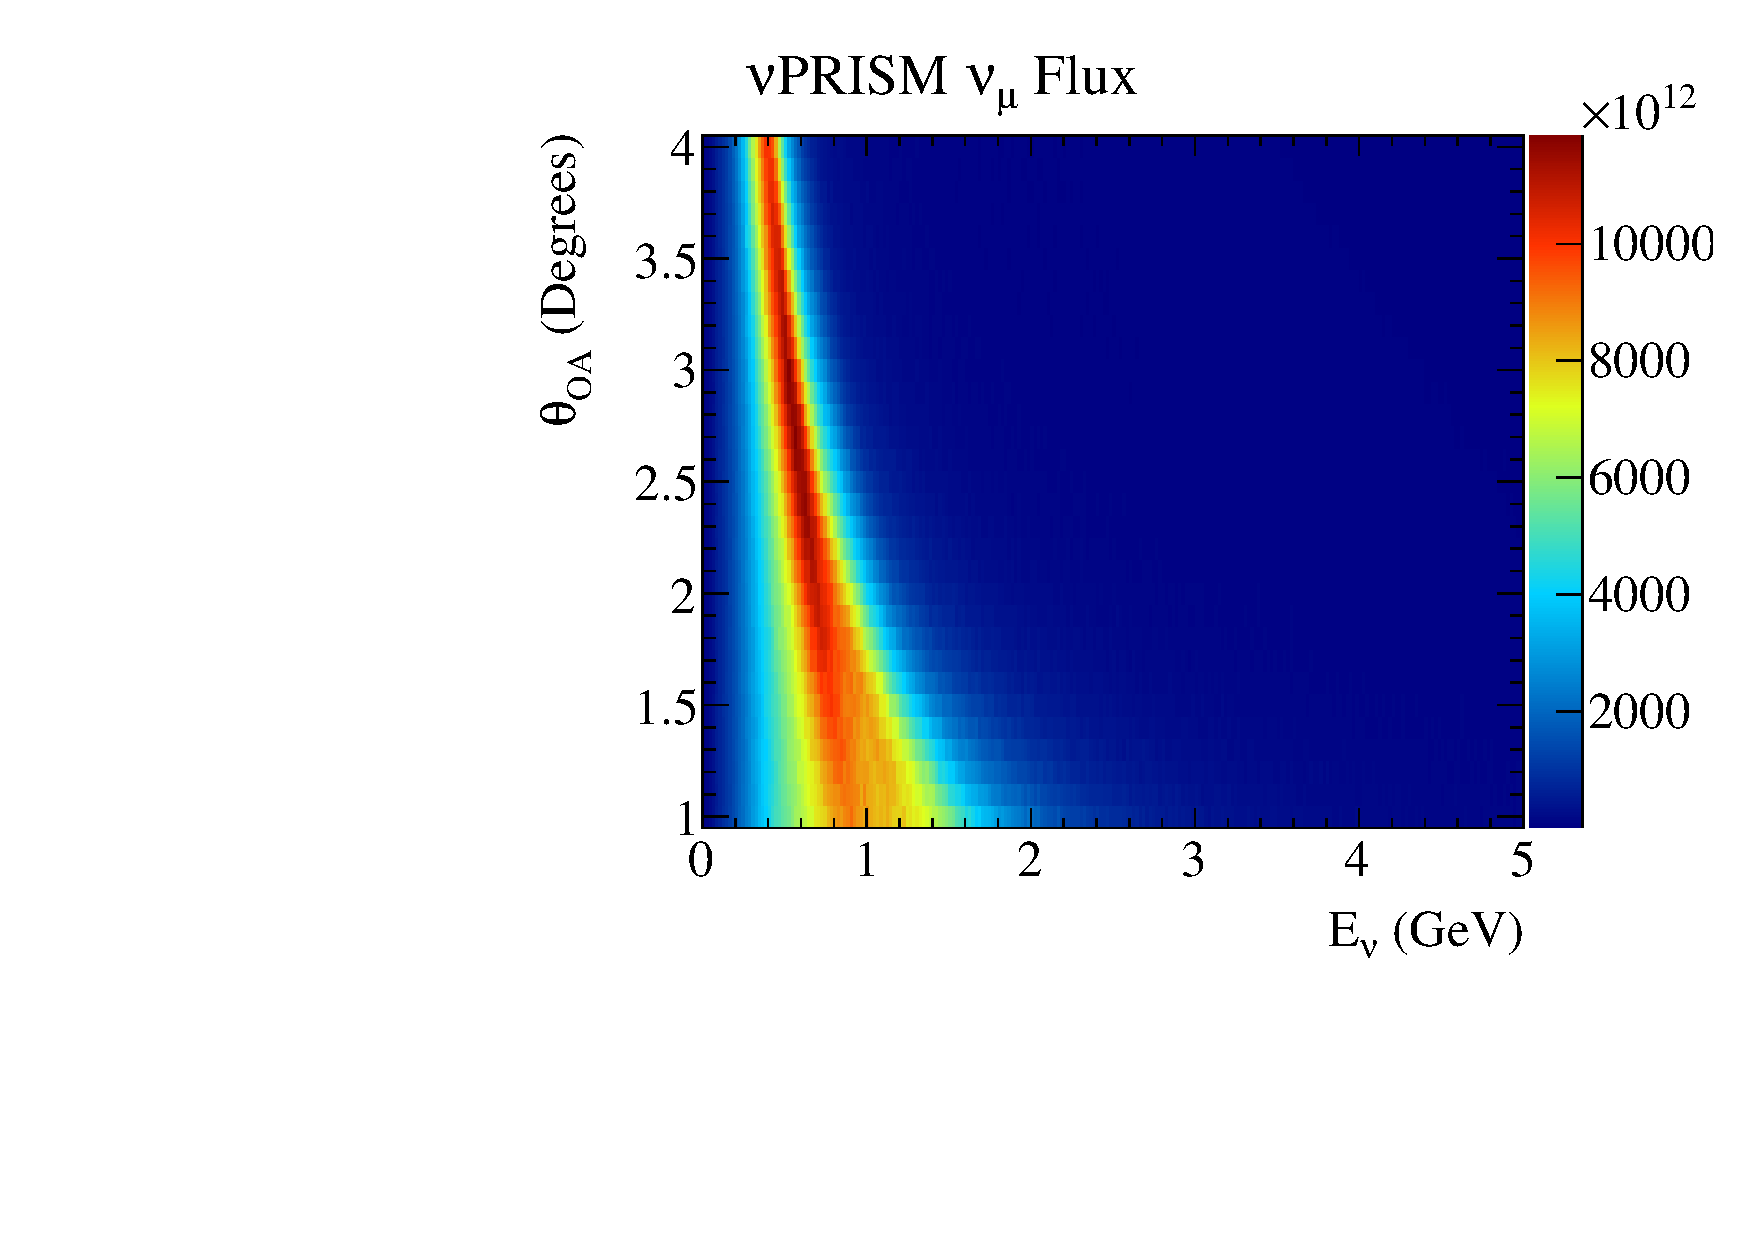
\includegraphics[width=0.45\textwidth]{figures/nuprism_oa_enu_numu.pdf}
  \caption{The $\nu_{\mu}$ flux spectra in the J-PARC neutrino beam for a range of off-axis angles.}
  \label{fig:off-axis}
  \end{center}
\end{figure}

{\color{red} \it Need to connect experiment which covers off-axis angles to the nuPRISM concept. No real association yet?  }
{\color{red} \it No statement of "need" of monochromatic as resolving the issues  }

{\color{red} \it Reference later section in paper. Need to include this in the concept but allow enough for future paper.   }
A detector with a base line of $\sim1$~km and off-axis spectra may also be used to search for short-baseline neutrino oscillations
consistent with the LSND~\cite{Athanassopoulos:1996jb} or MiniBooNE~\cite{Aguilar-Arevalo:2013pmq} $\nu_{e}$ appearance anomalies.  
The observed excess in MiniBooNE may arise from 
oscillations associated with one or more sterile neutrinos, or more mundane mis-modeling of neutral current (NC) or charged current (CC) 
cross sections.  If sterile neutrinos are the cause of the excess, the energy dependence of the oscillations will lead to a 
unique pattern over the range of off-axis spectra that can be differentiated from mis-modelled interactions.

\subsection{The electron neutrino cross-section}
{\color{red} \it Move this discussion earlier to be closer connected to the error budget in CP measurements }
The neutrino oscillation channel used to probe for CP violation is $\nu_{\mu}(\bar{\nu}_{\mu})\rightarrow\nu_{e}(\bar{\nu}_{e})$.
While the beam observed by near detectors is $\sim99\%$ $\nu_{\mu}(\bar{\nu}_{\mu})$, the signal at the far detector
is $\nu_{e}(\bar{\nu}_{e})$.  Hence uncertainties in the relative cross-section of muon and electron neutrinos are also
critical.  Electron neutrinos of energy $~1$ GeV can be produced in the decays of muons, however, in conventional beams a
beam dump stops most muons before they decay.
In the absence of a stored muon beam, the study of the $\nu_{e}$ cross sections at $~1$ GeV is challenging.  Since the
$\nu_{e}$ component of the beam is only $~1\%$, a detector with a large fiducial mass and very pure particle identification 
capabilities is required.  Recent improvements in electron and $\pi^{0}$ separation in water Cherenkov detectors, and the capability 
of water Cherenkov detectors to scale to very large fiducial masses suggest that they can be used to measure the electron
neutrino cross section with unprecedented precision in a conventional neutrino beam.


